\documentclass[a4paper, 12pt]{extreport}
\usepackage[utf8]{inputenc}
\usepackage[english,russian]{babel}
\usepackage{amssymb,amsfonts,amsmath,mathtext,cite,enumerate,float}
\usepackage{pgfplots}
\usepackage{graphicx}
\usepackage[inkscapeformat=png]{svg}
\usepackage{tocloft}
\usepackage{listings}
\usepackage{caption}
\usepackage{tempora}
\usepackage{titlesec}
\usepackage{setspace}
\usepackage{geometry}
\usepackage{indentfirst}
\usepackage{pdfpages}
\usepackage{enumerate,letltxmacro}
\usepackage{threeparttable}
\usepackage{hyperref}
\usepackage{flafter}
\usepackage{enumitem}
\usepackage{multirow}
\usepackage{mathtools}
\usepackage{longtable}
\usepackage[figure,table]{totalcount}
\usepackage{lastpage}

\lstdefinestyle{python}{
	language={Python},
	basicstyle=\footnotesize\ttfamily,
	frame=single,
	tabsize=4,	
	breaklines=true
}

\setlist{nosep}
\hypersetup{pdfborder=0 0 0}

\newcommand{\ssr}[1]{\begin{center}\LARGE\bfseries{#1}\end{center} \addcontentsline{toc}{chapter}{#1}  }

\makeatletter
\renewcommand\LARGE{\@setfontsize\LARGE{22pt}{20}}
\renewcommand\Large{\@setfontsize\Large{20pt}{20}}
\renewcommand\large{\@setfontsize\large{16pt}{20}}
\makeatother

\RequirePackage{titlesec}
\titleformat{\chapter}[block]{\hspace{\parindent}\large\bfseries}{\thechapter}{0.5em}{\large\bfseries\raggedright}
\titleformat{name=\chapter,numberless}[block]{\hspace{\parindent}}{}{0pt}{\large\bfseries\centering}
\titleformat{\section}[block]{\hspace{\parindent}\large\bfseries}{\thesection}{0.5em}{\large\bfseries\raggedright}
\titleformat{\subsection}[block]{\hspace{\parindent}\large\bfseries}{\thesubsection}{0.5em}{\large\bfseries\raggedright}
\titleformat{\subsubsection}[block]{\hspace{\parindent}\large\bfseries}{\thesubsection}{0.5em}{\large\bfseries\raggedright}
\titlespacing{\chapter}{12.5mm}{-22pt}{10pt}
\titlespacing{\section}{12.5mm}{10pt}{10pt}
\titlespacing{\subsection}{12.5mm}{10pt}{10pt}
\titlespacing{\subsubsection}{12.5mm}{10pt}{10pt}

\makeatletter
\renewcommand{\@biblabel}[1]{#1.}
\makeatother

\geometry{left=30mm}
\geometry{right=10mm}
\geometry{top=20mm}
\geometry{bottom=20mm}

\onehalfspacing

\renewcommand{\theenumi}{\arabic{enumi}}
\renewcommand{\labelenumi}{\arabic{enumi}\text{)}}
\renewcommand{\theenumii}{.\arabic{enumii}}
\renewcommand{\labelenumii}{\asbuk{enumii}\text{)}}
\renewcommand{\theenumiii}{.\arabic{enumiii}}
\renewcommand{\labelenumiii}{\arabic{enumi}.\arabic{enumii}.\arabic{enumiii}.}

\renewcommand{\cftchapleader}{\cftdotfill{\cftdotsep}}

\addto\captionsrussian{\renewcommand{\figurename}{Рисунок}}
\DeclareCaptionLabelSeparator{dash}{~---~}
\captionsetup{labelsep=dash}

\captionsetup[figure]{justification=centering,labelsep=dash}
\captionsetup[table]{labelsep=dash,justification=raggedright,singlelinecheck=off}
\captionsetup[lstlisting]{labelsep=dash,justification=raggedright,singlelinecheck=off}

\newcommand{\floor}[1]{\lfloor #1 \rfloor}

\pgfplotsset{width=0.85\linewidth, height=0.5\columnwidth}

\linespread{1.3}

\parindent=1.25cm

\def\labelitemi{---}
\setlist[itemize]{leftmargin=1.25cm, itemindent=0.65cm}
\setlist[enumerate]{leftmargin=1.25cm, itemindent=0.55cm}

\newcommand{\specialcell}[2][c]{\begin{tabular}[#1]{@{}c@{}}#2\end{tabular}}
\frenchspacing


\begin{document}
\begin{titlepage}
	\newgeometry{pdftex, left=2cm, right=2cm, top=2.5cm, bottom=2.5cm}
	\fontsize{12pt}{12pt}\selectfont
	\noindent\begin{tabular}{|c|c|}	\hline
	\noindent\begin{minipage}{0.15\textwidth}
		
\includegraphics[width=\linewidth]{tools/logo.png}
	\end{minipage} &
	\noindent\begin{minipage}{0.85\textwidth}\centering
		\textbf{\newline Министерство науки и высшего образования Российской Федерации}\\
		\textbf{Федеральное государственное бюджетное образовательное учреждение высшего образования}\\
		\textbf{«Московский государственный технический университет имени Н.Э.~Баумана}\\
		\textbf{(национальный исследовательский университет)»}\\
		\textbf{(МГТУ им. Н.Э.~Баумана)}
	\end{minipage} \\
	\hline	\end{tabular}\newline\newline\newline
	\noindent ФАКУЛЬТЕТ \underline{«Информатика и системы управления»} \newline\newline
	\noindent КАФЕДРА \underline{«Программное обеспечение ЭВМ и информационные технологии»}\newline\newline\newline\newline\newline\newline

	\noindent\begin{minipage}{1.0\textwidth}\centering
		\Large\textbf{       Лабораторная работа №6}
		\end{minipage}
		
	\noindent\begin{minipage}{1.0\textwidth}\centering
		\textbf{\newline}	
		\end{minipage}

	\noindent\begin{minipage}{1.0\textwidth}\centering
		\Large\textbf{по дисциплине «Анализ алгоритмов»}	
		\end{minipage}
		
	\noindent\begin{minipage}{1.0\textwidth}\centering
		\Large\textbf{\newline\newline\newline\newline}	
		\end{minipage}
		
	\noindent\textbf{Тема} \underline{Задача коммивояжёра}\newline\newline
	\textbf{Студент} \underline{Тузов Даниил Александрович}\newline\newline
	\textbf{Группа} \underline{ИУ7-52Б}\newline\newline
	\textbf{Преподаватель} \underline{Строганов Дмитрий Владимирович}
	
	\begin{center}
		\vfill
		Москва, \the\year~г.
	\end{center}
	\restoregeometry
	\clearpage
\end{titlepage}



\setlength{\cftbeforetoctitleskip}{-4mm}
\renewcommand{\contentsname}{\makebox[\textwidth][c]{\largeСОДЕРЖАНИЕ}}
\tableofcontents
\setcounter{page}{2}

\clearpage\ssr{ВВЕДЕНИЕ}

В 6 лабораторной работе рассматриваются методы решения задачи коммивояжёра.

Целью работы является разработка ПО, решающего задачу коммивояжёра. Для достижения поставленной цели необходимо 
решить следующие задачи:
\begin{itemize}
	\item[---] сформулировать задачу коммивояжёра;
	\item[---] рассмотреть метод решения задачи с помощью алгоритма полного перебором;
	\item[---] рассмотреть метод решения задачи с помощью муравьиного алгоритма;
	\item[---] реализовать алгоритмы;
	\item[---] сравнить время выполнения влгоритмов;
	\item[---] выполнить параметризацию;
	\item[---] обосновать полученные результаты.
\end{itemize}

\chapter{Аналитическая часть}

В этой части сформулировано условие задачи коммивояжёра, а также приведены теоретические аспекты алгоритмов полного 
перебора и муравьиного алгоритма для решения задачи коммивояжёра.

\section{Задачи коммивояжера}

Пусть задан граф $G = (V, E)$, где $V$ -- множество вершин ($|V| = n$), а $E$ -- множество ребер ($|E| = m$). Каждое ребро $(i, j) 
\in E$ имеет длину $c_{ij}$, которая задается матрицей расстояний $C = \|c_{ij}\|$. Если между вершинами $i$ и $j$ нет ребра, 
соответствующий элемент матрицы считается равным бесконечности ($c_{ij} = \infty$)~\cite{comi}.

Требуется найти такой путь в графе, который содержит все вершины и при этом его длина минимальна.

\section{Алгоритм полного перебора}

Один из возможных алгоритмов решения задачи коммивояжёра состоит в том, чтобы перебрать все возможные перестановки
номеров вершин в графе. При этом для каждой перестановки считается длина пути. Среди найденных длин выбирается 
минимальная. Сложность такого алгоритма $O(N!)$, где N -- количество вершин в графе~\cite{comi}.

\section{Муравьиный алгоритм}

Муравьиный алгоритм --- это метод решения задачи коммивояжера, основанный на моделировании поведения муравьиной 
колонии. Каждый муравей прокладывает маршрут, используя информацию о феромонах, оставленных другими 
муравьями на графе. В процессе движения муравей оставляет феромон на своем пути, чтобы другие могли ориентироваться на 
него. Постепенно феромоны на оптимальном маршруте накапливаются, так как он используется наиболее часто.~\cite{shtovba}

Характеристики муравья:
\begin{itemize}
    \item[---] зрение -- муравей способен оценивать длину ребер;
    \item[---] память -- запоминает посещенные вершины;
    \item[---] обоняние -- реагирует на феромоны, оставленные другими муравьями.
\end{itemize}

Для оценки привлекательности перехода используется функция~\eqref{d_func}:
\begin{equation}
    \label{d_func}
    \eta_{ij} = \frac{1}{D_{ij}},
\end{equation}
где $D_{ij}$ — расстояние между вершинами $i$ и $j$.

Вероятность перехода муравья $k$ из текущей вершины $i$ в вершину $j$ рассчитывается по формуле~\eqref{posib}:
\begin{equation}
    \label{posib}
    P_{kij} = 
    \begin{cases}
        \frac{\tau_{ij}^a \eta_{ij}^b}{\sum_{q \in J_{ik}} \tau_{iq}^a \eta_{iq}^b}, & \text{если вершина $j$ еще не посещена муравьем $k$,} \\
        0, & \text{иначе,}
    \end{cases}
\end{equation}
где:
\begin{itemize}
    \item $a$ — параметр влияния феромона;
    \item $b$ — параметр влияния длины пути;
    \item $\tau_{ij}$ — количество феромонов на ребре $(i, j)$;
    \item $\eta_{ij}$ — видимость (обратная расстоянию).
\end{itemize}

В конце дня уровень феромонов на ребрах обновляется по формуле~\eqref{update_phero_1}:
\begin{equation}
    \label{update_phero_1}
    \tau_{ij}(t+1) = (1-p)\tau_{ij}(t) + \Delta \tau_{ij},
\end{equation}
где $p$ — коэффициент испарения феромона, а $\Delta \tau_{ij}$ определяется как:

\begin{equation}
    \label{update_phero_2}
    \Delta \tau_{ij} = \sum_{k=1}^N \Delta \tau_{ij}^k,
\end{equation}

\begin{equation}
    \label{update_phero_3}
    \Delta \tau_{ij}^k = 
    \begin{cases}
        \frac{Q}{L_k}, & \text{если ребро $(i, j)$ посещено муравьем $k$,} \\
        0, & \text{иначе,}
    \end{cases}
\end{equation}

где $Q$ — параметр, связанный с длиной оптимального пути, а $L_k$ — длина маршрута муравья $k$.

\section{Вывод}

В этой части была сформулирована задача коммивояжёра и рассмотрены теоретические аспекты ее решения.

\chapter{Конструкторская часть}

В этой части представлены описания алгоритмов.

\section{Описание алгоритма полного перебора}

На вход алгоритму подается матрица \texttt{mat} на выходе длина минимального пути и сам минимальный путь.

На рисунке~\ref{scheme:full} приведено описание алгоритма полного перебора.
	
\begin{figure}[h]
	\centering
	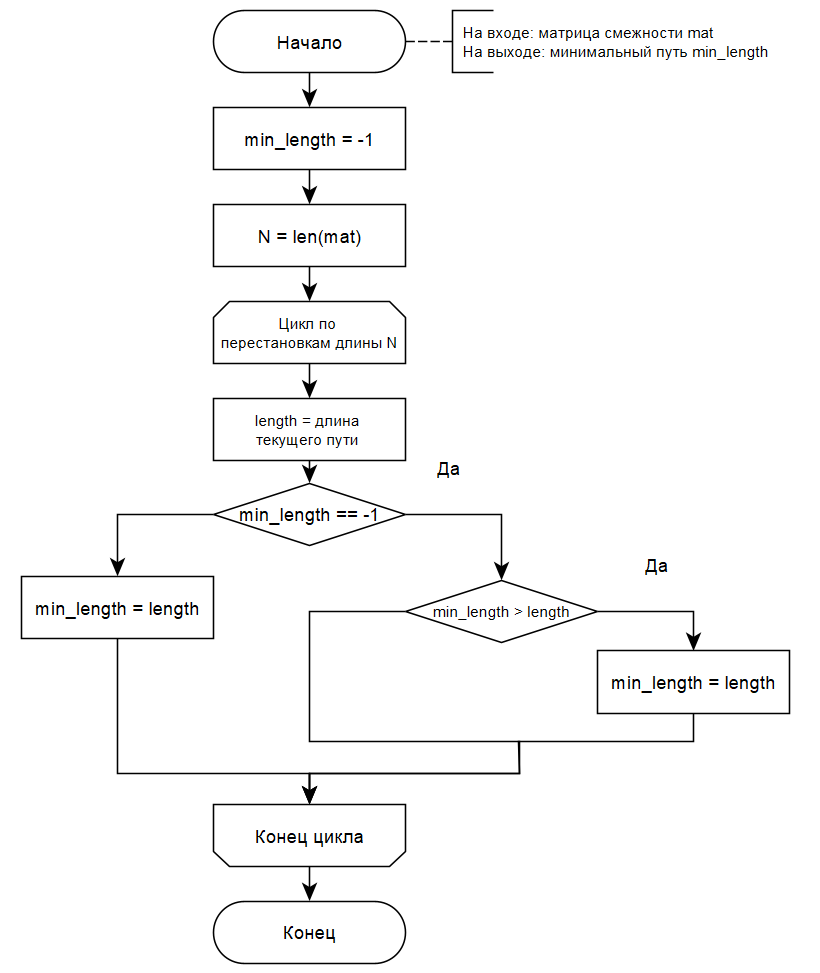
\includegraphics[scale=0.7]{tools/full.png}
	\caption{Описание алгоритма полного перебора}
	\label{scheme:full}
\end{figure}

\section{Описание муравьиного алгоритма}

На вход алгоритму подается матрица \texttt{mat} и коэффициенты $\alpha$, $\rho$ и $t_{max}$ на выходе длина минимального 
пути и сам минимальный путь.

На рисунке~\ref{scheme:full} приведено описание муравьиного алгоритма.

\begin{figure}[h]
	\centering
	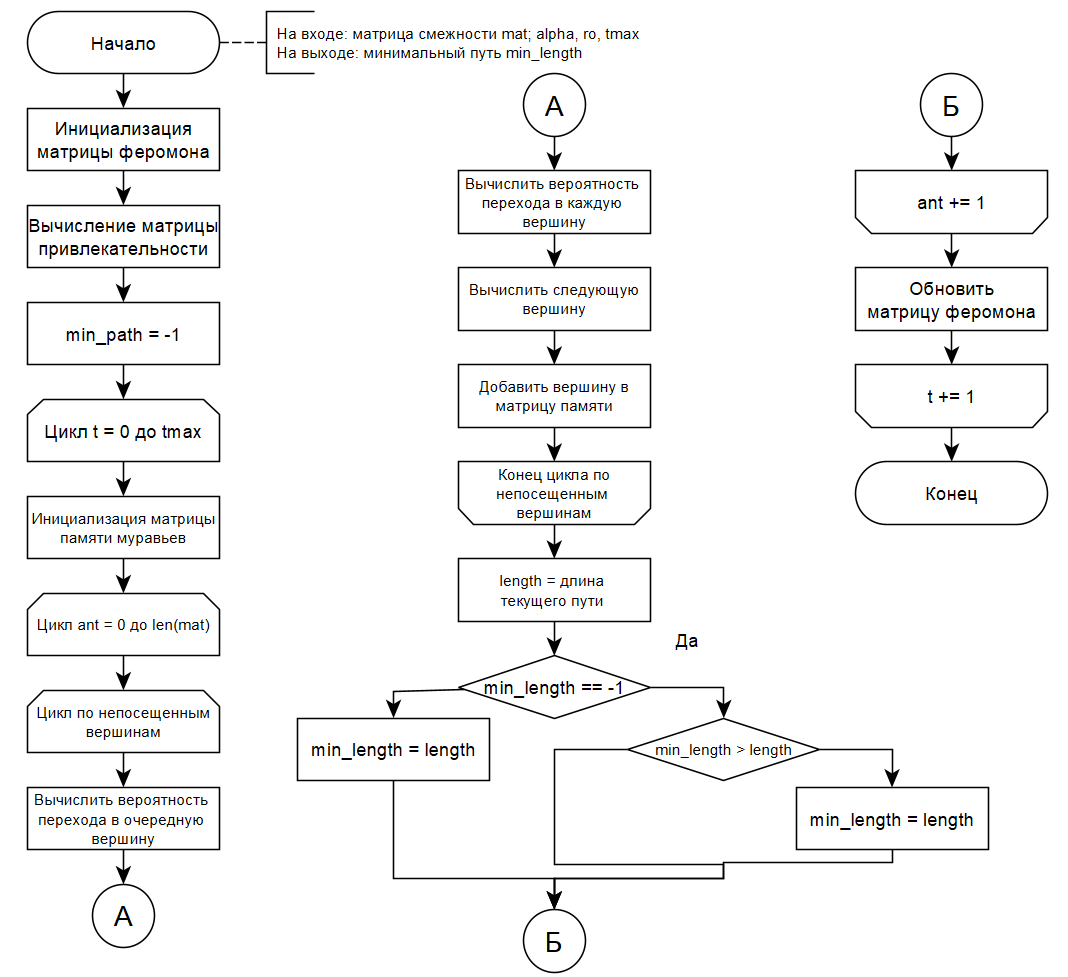
\includegraphics[scale=0.7]{tools/ant.png}
	\caption{Описание муравьиного алгоритма}
	\label{scheme:ant}
\end{figure}

\section{Вывод}
В этом разделе на основе теоретических аспектов были представлены описания алгоритма полного перебора и муравьиного
алгоритма.

\chapter{Технологическая часть}

В этом разделе обоснованы средства реализации, а так же представлены реализации алгоритмов и функциональные тесты.

\section{Средства реализации}

Для реализации алгоритмов в этой лабораторной работы был выбран язык $Python$~\cite{python3}, потому что в нем нет 
автоматического сборщика мусора.

\section{Реализация алгоритмов}

В листингах~\ref{lst:full}---\ref{lst:ant} представлены коды написанных алгоритмов.

\begin{lstlisting}[style=python, label=lst:full,caption=Алгоритм полного перебора]
def standard_alg(mat):
    n = len(mat)
    vertexes = [ i + 1 for i in range(n) ]
    min_path_len = -1
    best_path = tuple()
    for path in permutations(vertexes):
        path_len = 0
        for i in range(len(path) - 1):
            a, b = path[i], path[i + 1]
            path_len += mat[a - 1][b - 1]
        if min_path_len == -1 or min_path_len > path_len:
            min_path_len = path_len
            best_path = path
    return list(best_path), min_path_len
\end{lstlisting}

\begin{lstlisting}[style=python, label=lst:ant,caption=Муравьиный алгоритм]
def ant_alg(mat, alpha, ro, t_max):
    n, q = len(mat), calc_q(mat)
    pheromone = init_pheromone(n)
    attract = init_attract(mat)
    min_path_len = -1
    best_path = list()
    for t in range(t_max):
        memory = init_memory(n)
        for ant in range(n):
            while len(memory[ant]) != n:
                p = calc_p(pheromone, attract, memory[ant], n, alpha)
                memory[ant].append(calc_next(p))
            path_len = calc_length(mat, memory[ant])
            if min_path_len == -1 or min_path_len > path_len:
                min_path_len = path_len
                best_path = memory[ant]
        pheromone = update_pheromone(mat, memory, pheromone, q, ro)
    for i in range(len(best_path)):
        best_path[i] += 1
    return best_path, min_path_len

def calc_q(mat):
    n, q = len(mat), 0
    for i in range(n):
        for j in range(n):
            if i != j:
                q += mat[i][j]
    return q / (n ** 3 - n)

def init_pheromone(n):
    return [[1 for i in range(n)] for j in range(n)]

def init_attract(mat):
    return [[(1 / mat[i][j] if i != j else 0) for i in range(len(mat))] for j in range(len(mat))]

def init_memory(n):
    memory = list()
    for i in range(n):
        memory.append([i])
    return memory

def calc_p(pheromon, attract, memory, n, alpha):
    beta = 1 - alpha
    p = [0] * n
    for new_pos in range(n):
        if new_pos in memory:
            p[new_pos] = 0
        else:
            last_pos = memory[-1]
            p[new_pos] = pheromon[last_pos][new_pos] ** beta * attract[last_pos][new_pos] ** alpha
    psum = sum(p)
    for i in range(n):
        p[i] /= psum
    return p

def calc_next(p):
    point = random()
    i = 0
    while i < len(p):
        if point - p[i] < 0:
            return i
        point -= p[i]
        i += 1
    return len(p)

def calc_length(mat, path):
    length = 0
    for i in range(len(path) - 1):
        a, b = path[i], path[i + 1]
        length += mat[a][b]
    return length

def update_pheromone(mat, memory, pheromone, q, ro):
    n = len(mat)
    for i in range(n):
        for j in range(n):
            delta = 0
            for ant in range(n):
                length = calc_length(mat, memory[ant])
                delta += q / length
            pheromone[i][j] = pheromone[i][j] * (1 - ro) + delta
            if pheromone[i][j] < 0.01:
                pheromone[i][j] = 0.01
    return pheromone
\end{lstlisting}

\section{Функциональные тесты}

В таблице~\ref{tbl:funcs} представлены результаты тестирования программы для алгоритма полного перебора.

\clearpage\begin{table}[h]
	\begin{center}
	\caption{\label{tbl:funcs} Функциональные тесты}
	\begin{tabular}{|c|c|c|}
		\hline
		Матрица смежности & Ожидаемый результат  & Статус
		\\ \hline
		$\begin{pmatrix}
		0 & 16 & 10 & 14 & 4 & 12 & 14 & 20 \\
		18 & 0 & 6 & 2 & 13 & 6 & 18 & 13 \\
		14 & 16 & 0 & 10 & 18 & 9 & 1 & 15 \\ 
		11 & 17 & 3 & 0 & 15 & 3 & 2 & 4 \\
		2 & 14 & 12 & 5 & 0 & 12 & 3 & 14 \\
		5 & 1 & 9 & 10 & 20 & 0 & 1 & 15 \\
		11 & 8 & 16 & 10 & 15 & 13 & 0 & 18 \\
		11 & 20 & 3 & 2 & 12 & 13 & 20 & 0
		\end{pmatrix}$ & [5, 1, 6, 2, 4, 8, 3, 7], 25 & ОК
		\\ \hline
		$\begin{pmatrix}
		0 & 20 & 7 & 6 & 17 & 9 & 20 & 20 & 14 \\
		8 & 0 & 6 & 12 & 1 & 2 & 12 & 20 & 18 \\
		19 & 7 & 0 & 12 & 19 & 5 & 20 & 7 & 14 \\
		2 & 9 & 4 & 0 & 13 & 10 & 14 & 3 & 20 \\
		13 & 20 & 1 & 10 & 0 & 17 & 8 & 5 & 20 \\
		9 & 13 & 8 & 16 & 6 & 0 & 7 & 13 & 19 \\
		15 & 4 & 7 & 3 & 17 & 1 & 0 & 14 & 5 \\
		19 & 1 & 9 & 20 & 1 & 6 & 15 & 0 & 17 \\
		17 & 19 & 9 & 15 & 4 & 6 & 16 & 4 & 0
		\end{pmatrix}$ & [9, 8, 2, 5, 3, 6, 7, 4, 1], 24 & ОК
		\\ \hline
		$\begin{pmatrix}
		0 & 16 & 11 & 8 & 10 & 4 & 12 & 4 & 9 & 7 \\
		4 & 0 & 12 & 5 & 12 & 13 & 19 & 2 & 17 & 14 \\
		1 & 2 & 0 & 9 & 18 & 15 & 16 & 19 & 19 & 2 \\
		5 & 19 & 17 & 0 & 18 & 8 & 7 & 7 & 4 & 1 \\
		12 & 17 & 2 & 20 & 0 & 13 & 20 & 20 & 6 & 11 \\
		16 & 4 & 8 & 16 & 5 & 0 & 3 & 17 & 2 & 17 \\
		9 & 12 & 9 & 7 & 11 & 14 & 0 & 7 & 19 & 6 \\
		11 & 20 & 5 & 9 & 10 & 19 & 19 & 0 & 13 & 17 \\
		19 & 16 & 12 & 19 & 16 & 13 & 9 & 4 & 0 & 13 \\
		13 & 8 & 4 & 8 & 20 & 7 & 12 & 14 & 12 & 0
		\end{pmatrix}$ & [5, 3, 1, 6, 9, 7, 4, 10, 2, 8], 36 & ОК
		\\ \hline
	\end{tabular}
	\end{center}
\end{table}


\section{Вывод}

В этом разделе на основе описаний алгоритмов были написаны и представлены коды алгоритмов. Помимо кодов
представлены функциональные тесты, на которых был протестирован алгоритм полного перебора.

\chapter{Исследовательская часть}

В этом разделе приведен график со сравнением времени работы алгоритмов на графах с разным количеством вершин, а так же
представлен результат параметризации муравьиного алгоритма.

\section{Технические характеристики ЭВМ}

Все замеры проводились на ЭВМ, характеристики которой приведены ниже:
\begin{itemize}
	\item[---] процессор -- 12th Gen Intel(R) Core(TM) i5-12450H 2.00 ГГц;
	\item[---] оперативная память -- 16,0 ГБ;
	\item[---] тип системы -- 64-разрядная операционная система, процессор x64;
	\item[---] операционная система -- Windows 11;
	\item[---] версия ОС -- 23H2;
	\item[---] 12 логических ядер.
\end{itemize}

\section{Сравнение времени работы}

Время выполнения работы алгоритмов представлено в секундах. Проводилось 10 замеров. Результаты представлены в 
таблице~\ref{tbl:all_time_cmp} и на рисунке~\ref{graph}.

\begin{table}[h]
	\begin{center}
	\caption{\label{tbl:all_time_cmp} Сравнение алгоритмов по времени выполнения}
	\begin{tabular}{|l|l|l|}
		\hline
		Количество вершин & Алгоритм полного перебора & Муравьиный алгоритм \\ 
		\hline
		2 & 0 & 0.002 \\ 
		\hline
		3 & 0 & 0.002 \\ 
		\hline
		4 & 0 & 0.008 \\ 
		\hline
		5 & 0 & 0.013 \\ 
		\hline
		6 & 0 & 0.023 \\ 
		\hline
		7 & 0 & 0.039 \\ 
		\hline
		8 & 0.02 & 0.059 \\ 
		\hline
		9 & 0.15 & 0.086 \\ 
		\hline
		10 & 1.46 & 0.098 \\ 
		\hline
	\end{tabular}
	\end{center}
\end{table}

\clearpage\begin{figure}[h]
	\centering
	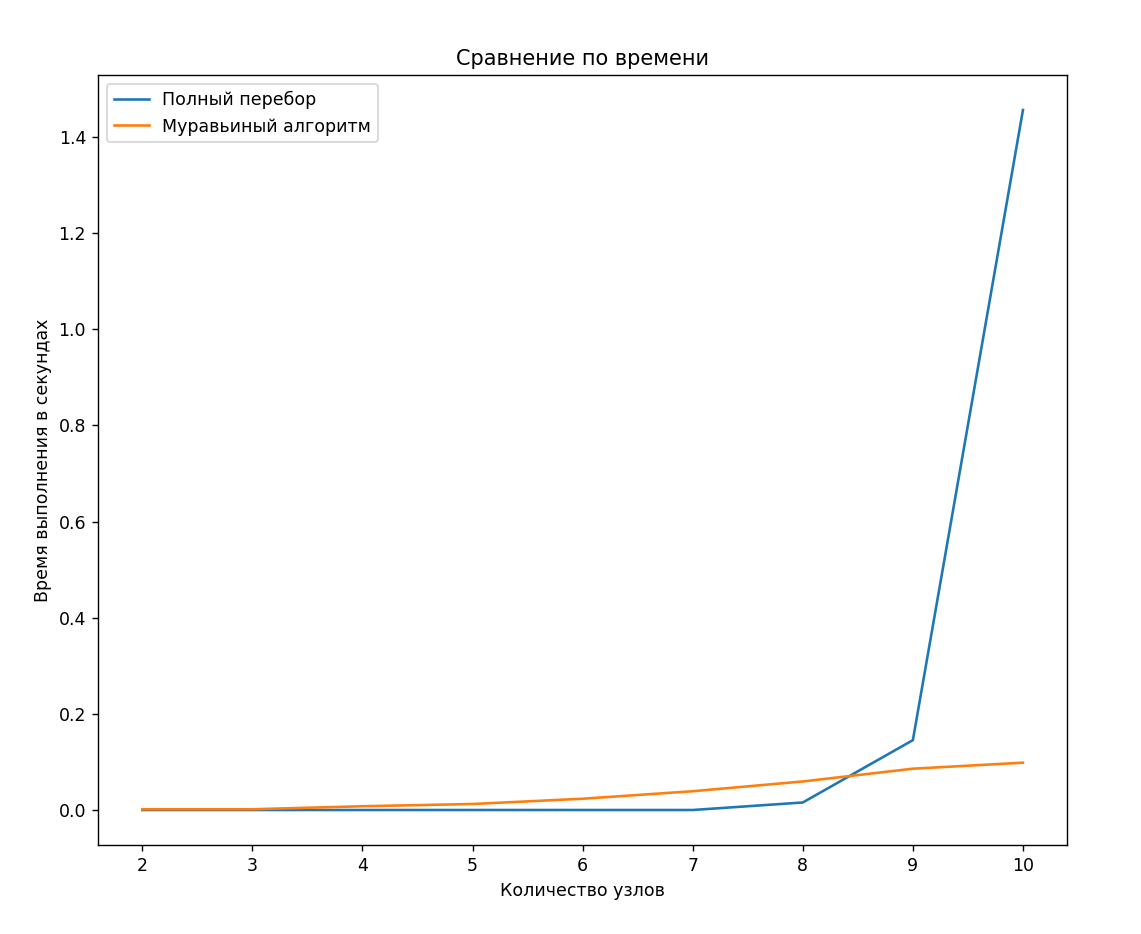
\includegraphics[scale=0.7]{tools/graph.png}
	\caption{Сравнение алгоритмов по времени выполнения}
	\label{graph}
\end{figure}

\section{Параметризация муравьиного алгоритма}

Параметризация выполнялась для 3 графов, представленных в технологической части в разделе с функциональными тестами.
Разультат параметризации представлен в приложении А.

\section{Вывод}

В результате сравнения алгоритмов по времени сделан вывод, что муравьиный алгоритм проигрывает для графа с количеством
вершин меньшим 9. Начиная с количества узлов равным 9, муравьиный алгоритм превосходит алгоритм полного перебора. 
Наилучшими параметрами параметризации являются $\alpha = 0.75$, $\rho = 0.5$, $t_{max} = 2000$.

\clearpage\ssr{ЗАКЛЮЧЕНИЕ}

В ходе выполнения лабораторной работы поставленная цель была достигнута. Были решены все задачи:
\begin{itemize}
	\item[---] сформулирована задача коммивояжёра;
	\item[---] рассмотрены методы решения задачи коммивояжера;
	\item[---] реализованы алгоритмы;
	\item[---] проведено сравнение алгоритмов по времени;
	\item[---] выполнена параметризация для муравьиного алгоритма;
	\item[---] обоснованы полученные результаты.
\end{itemize}

\addcontentsline{toc}{chapter}{СПИСОК ИСПОЛЬЗОВАННЫХ ИСТОЧНИКОВ}
\renewcommand{\bibname}{СПИСОК ИСПОЛЬЗОВАННЫХ ИСТОЧНИКОВ}
\begin{thebibliography}{}
	\bibitem{comi}  Меламед, Игорь Ильич and Сергеев, С И and Сигал, Израиль Хаимович. Задача коммивояжера. Вопросы теории. --- Автоматика и телемеханика, 1989, с.3-33 (дата обращения: 09.12.2024)
	\bibitem {shtovba} Штовба С.Д. Муравьиные алгоритмы. --- Exponenta Pro. Математика в приложениях, 2003, с.70-75 
(дата обращения: 09.12.2024)
	\bibitem{python3} Язык Python / [Электронный ресурс] // Режим доступа: https://docs.python.org/3/index.html  (дата 
обращения: 09.12.2024)
	\bibitem{random}Библиотека random / [Электронный ресурс] // Режим доступа: https://\\docs.python.org/3/library/
random.html (дата обращения: 09.12.2024)
	\bibitem{time} Библиотека time  / [Электронный ресурс] // Режим доступа: https://docs.python.org/3/library/time.html 
(дата обращения: 09.12.2024)
	\bibitem{plot} Библиотека matplotlib / [Электронный ресурс] // Режим доступа: https://\\matplotlib.org  (дата обращения: 
09.12.2024)
\end{thebibliography}

\clearpage\ssr{ПРИЛОЖЕНИЕ А}

\end{document}